\documentclass[twoside]{book}

% Packages required by doxygen
\usepackage{fixltx2e}
\usepackage{calc}
\usepackage{doxygen}
\usepackage[export]{adjustbox} % also loads graphicx
\usepackage{graphicx}
\usepackage[utf8]{inputenc}
\usepackage{makeidx}
\usepackage{multicol}
\usepackage{multirow}
\PassOptionsToPackage{warn}{textcomp}
\usepackage{textcomp}
\usepackage[nointegrals]{wasysym}
\usepackage[table]{xcolor}

% Font selection
\usepackage[T1]{fontenc}
\usepackage[scaled=.90]{helvet}
\usepackage{courier}
\usepackage{amssymb}
\usepackage{sectsty}
\renewcommand{\familydefault}{\sfdefault}
\allsectionsfont{%
  \fontseries{bc}\selectfont%
  \color{darkgray}%
}
\renewcommand{\DoxyLabelFont}{%
  \fontseries{bc}\selectfont%
  \color{darkgray}%
}
\newcommand{\+}{\discretionary{\mbox{\scriptsize$\hookleftarrow$}}{}{}}

% Page & text layout
\usepackage{geometry}
\geometry{%
  letterpaper,%
  top=2.5cm,%
  bottom=2.5cm,%
  left=2.5cm,%
  right=2.5cm%
}
\tolerance=750
\hfuzz=15pt
\hbadness=750
\setlength{\emergencystretch}{15pt}
\setlength{\parindent}{0cm}
\setlength{\parskip}{3ex plus 2ex minus 2ex}
\makeatletter
\renewcommand{\paragraph}{%
  \@startsection{paragraph}{4}{0ex}{-1.0ex}{1.0ex}{%
    \normalfont\normalsize\bfseries\SS@parafont%
  }%
}
\renewcommand{\subparagraph}{%
  \@startsection{subparagraph}{5}{0ex}{-1.0ex}{1.0ex}{%
    \normalfont\normalsize\bfseries\SS@subparafont%
  }%
}
\makeatother

% Headers & footers
\usepackage{fancyhdr}
\pagestyle{fancyplain}
\fancyhead[LE]{\fancyplain{}{\bfseries\thepage}}
\fancyhead[CE]{\fancyplain{}{}}
\fancyhead[RE]{\fancyplain{}{\bfseries\leftmark}}
\fancyhead[LO]{\fancyplain{}{\bfseries\rightmark}}
\fancyhead[CO]{\fancyplain{}{}}
\fancyhead[RO]{\fancyplain{}{\bfseries\thepage}}
\fancyfoot[LE]{\fancyplain{}{}}
\fancyfoot[CE]{\fancyplain{}{}}
\fancyfoot[RE]{\fancyplain{}{\bfseries\scriptsize Generated by Doxygen }}
\fancyfoot[LO]{\fancyplain{}{\bfseries\scriptsize Generated by Doxygen }}
\fancyfoot[CO]{\fancyplain{}{}}
\fancyfoot[RO]{\fancyplain{}{}}
\renewcommand{\footrulewidth}{0.4pt}
\renewcommand{\chaptermark}[1]{%
  \markboth{#1}{}%
}
\renewcommand{\sectionmark}[1]{%
  \markright{\thesection\ #1}%
}

% Indices & bibliography
\usepackage{natbib}
\usepackage[titles]{tocloft}
\setcounter{tocdepth}{3}
\setcounter{secnumdepth}{5}
\makeindex

% Hyperlinks (required, but should be loaded last)
\usepackage{ifpdf}
\ifpdf
  \usepackage[pdftex,pagebackref=true]{hyperref}
\else
  \usepackage[ps2pdf,pagebackref=true]{hyperref}
\fi
\hypersetup{%
  colorlinks=true,%
  linkcolor=blue,%
  citecolor=blue,%
  unicode%
}

% Custom commands
\newcommand{\clearemptydoublepage}{%
  \newpage{\pagestyle{empty}\cleardoublepage}%
}

\usepackage{caption}
\captionsetup{labelsep=space,justification=centering,font={bf},singlelinecheck=off,skip=4pt,position=top}

%===== C O N T E N T S =====

\begin{document}

% Titlepage & ToC
\hypersetup{pageanchor=false,
             bookmarksnumbered=true,
             pdfencoding=unicode
            }
\pagenumbering{alph}
\begin{titlepage}
\vspace*{7cm}
\begin{center}%
{\Large align2bed \\[1ex]\large 0.\+9 }\\
\vspace*{1cm}
{\large Generated by Doxygen 1.8.13}\\
\end{center}
\end{titlepage}
\clearemptydoublepage
\pagenumbering{roman}
\tableofcontents
\clearemptydoublepage
\pagenumbering{arabic}
\hypersetup{pageanchor=true}

%--- Begin generated contents ---
\chapter{Overview}
\label{index}\hypertarget{index}{}{\itshape align2bed} is a light-\/weight tool that extracts single nucleotide polymorphisms (S\+N\+Ps) from F\+A\+S\+TA alignments and saves them to a \href{http://zzz.bwh.harvard.edu/plink/index.shtml}{\tt plink} binary-\/format B\+ED file. It is fast and can process whole-\/genome data on a laptop in minutes. The F\+A\+S\+TA alignments should be in the format provided by the {\itshape Drosophila} Genome Nexus (\href{http://www.johnpool.net/genomes.html}{\tt http\+://www.\+johnpool.\+net/genomes.\+html}), i.\+e. the data for each line (or individual) are in a separate file with nucleotides in one line and without the customary F\+A\+S\+TA header. Each chromosome arm has its own set of files.

The sofware uses control files that list paths to each F\+A\+S\+TA file to be processed. An example data set is included to illustrate the necessary features of the data. One of the individuals must be marked as the reference, and it is also assumed that this reference is the outgroup. The reference genotypes are not included in the output. B\+ED format files require the S\+N\+Ps to be biallelic, so S\+N\+Ps that do not meet this criterion are not included as output. However, if a S\+NP is biallelic within the population (non-\/reference) sample, but both alleles are different from the outgroup, it is included. Names of such S\+N\+Ps are marked with \char`\"{}d\char`\"{} at the end (in the accompanying .bim file) to enable downstream filtering. In addition, S\+N\+Ps with outgroup missing are included but their names marked with \char`\"{}m\char`\"{} at the end. S\+NP names are \char`\"{}s\char`\"{} plus position, then \char`\"{}m\char`\"{} or \char`\"{}d\char`\"{} if applicable, then underscore (\char`\"{}\+\_\+\char`\"{}), then chromosome arm name.

While {\itshape align2bed} is tailored for the {\itshape Drosophila} Genome Nexus data, there are three ways it can be extended to similar data sets from other species. Data can be arranged to mimic the {\itshape Drosophila} set by treating chromosomes in groups of five. Alignment length can vary indefinitely. Furthermore, I wrote the program using a class that has wider applicability. Taking the {\itshape align2bed} source code as an exmaple, and reading the provided interface documentation, someone with even very limited experience in C++ can write software that applies to different data sets and hardware configurations. Finally, anyone who would like to extend functionality even further is welcome to modify the class implementation to suit their needs.

Neither {\itshape align2bed} itself nor the class used to implement it has any dependencies outside of the C++ S\+TL. Only a compiler capable of recognizing the C++11 standard is required. The implementation is multithreaded, with chromosome arms processed in parallel. Each thread allocates a 2\+Gb buffer to read the F\+A\+S\+TA files. The {\itshape align2bed} source can be easily modified to change the threading and memory allocation parameters (see included class documentation for details).

To compile, make sure you are in the directory with the source code files and run \begin{DoxyVerb}g++ align2bed.cpp sequence.cpp -o align2bed -O3 -march=native -std=c++11
\end{DoxyVerb}


then copy the binary where you need it. Run by typing {\ttfamily ./align2bed} in the directory with the binary and the data, or move into an appropriate /bin folder for global access. 
\chapter{Class Index}
\section{Class List}
Here are the classes, structs, unions and interfaces with brief descriptions\+:\begin{DoxyCompactList}
\item\contentsline{section}{\hyperlink{class_s_fparse}{S\+Fparse} \\*Sequence file parsing class }{\pageref{class_s_fparse}}{}
\end{DoxyCompactList}

\chapter{File Index}
\section{File List}
Here is a list of all documented files with brief descriptions\+:\begin{DoxyCompactList}
\item\contentsline{section}{\hyperlink{align2bed_8cpp}{align2bed.\+cpp} \\*Parsing D\+P\+GP }{\pageref{align2bed_8cpp}}{}
\item\contentsline{section}{\hyperlink{sequence_8cpp}{sequence.\+cpp} \\*Sequence and S\+NP file parsing and conversion }{\pageref{sequence_8cpp}}{}
\item\contentsline{section}{\hyperlink{sequence_8hpp}{sequence.\+hpp} \\*Sequence and S\+NP file parsing and conversion }{\pageref{sequence_8hpp}}{}
\end{DoxyCompactList}

\chapter{Class Documentation}
\hypertarget{class_s_fparse}{}\section{S\+Fparse Class Reference}
\label{class_s_fparse}\index{S\+Fparse@{S\+Fparse}}


Sequence file parsing class.  




{\ttfamily \#include $<$sequence.\+hpp$>$}

\subsection*{Public Member Functions}
\begin{DoxyCompactItemize}
\item 
\mbox{\Hypertarget{class_s_fparse_a6199b21081670322a0b0d7bbfeceb9a9}\label{class_s_fparse_a6199b21081670322a0b0d7bbfeceb9a9}} 
\hyperlink{class_s_fparse_a6199b21081670322a0b0d7bbfeceb9a9}{S\+Fparse} ()
\begin{DoxyCompactList}\small\item\em Default constructor. \end{DoxyCompactList}\item 
\hyperlink{class_s_fparse_a63162a0c3d8c855602796198854eb36f}{S\+Fparse} (const vector$<$ string $>$ \&in\+Fl\+Nam, const vector$<$ string $>$ \&line\+Names, const string \&ref\+Fl\+Nam, const string \&out\+Fl\+Nam, const string \&chr\+Nam, const unsigned short \&chr\+Num, const string \&in\+Fl\+Type, const string \&out\+Fl\+Type, const unsigned long \&alloc=2000000000\+U\+L)
\begin{DoxyCompactList}\small\item\em Constructor with vectors of names. \end{DoxyCompactList}\item 
\hyperlink{class_s_fparse_aa66f34c1f0db7451a191461f3f303137}{S\+Fparse} (const string \&file\+List, const string \&out\+Fl\+Nam, const string \&chr\+Nam, const unsigned short \&chr\+Num, const string \&in\+Fl\+Type, const string \&out\+Fl\+Type, const unsigned long \&alloc=2000000000\+U\+L)
\begin{DoxyCompactList}\small\item\em Constructor with file list and explicit types. \end{DoxyCompactList}\item 
\hyperlink{class_s_fparse_a7adee31d2eaa489b64e25f690348ce99}{S\+Fparse} (const string \&file\+List, const string \&out\+Fl\+Nam, const unsigned long \&alloc=2000000000\+U\+L)
\begin{DoxyCompactList}\small\item\em Constructor with file list. \end{DoxyCompactList}\item 
\mbox{\Hypertarget{class_s_fparse_a197d31f86dd544159fc8d8d79e36aaaf}\label{class_s_fparse_a197d31f86dd544159fc8d8d79e36aaaf}} 
\hyperlink{class_s_fparse_a197d31f86dd544159fc8d8d79e36aaaf}{$\sim$\+S\+Fparse} ()
\begin{DoxyCompactList}\small\item\em Destructor. \end{DoxyCompactList}\item 
\hyperlink{class_s_fparse_ae85a63a8883ec1c318cabdcb30398063}{S\+Fparse} (const \hyperlink{class_s_fparse}{S\+Fparse} \&in\+Obj)
\begin{DoxyCompactList}\small\item\em Copy constructor. \end{DoxyCompactList}\item 
\hyperlink{class_s_fparse}{S\+Fparse} \& \hyperlink{class_s_fparse_a5f7e978d765c8fb8735526fac38a301f}{operator=} (const \hyperlink{class_s_fparse}{S\+Fparse} \&in\+Obj)
\begin{DoxyCompactList}\small\item\em Copy assignement operator. \end{DoxyCompactList}\item 
\hyperlink{class_s_fparse_a9c3e1e6f6f687ecf61f046e1bcf5b61c}{S\+Fparse} (\hyperlink{class_s_fparse}{S\+Fparse} \&\&in\+Obj)
\begin{DoxyCompactList}\small\item\em Move constructor. \end{DoxyCompactList}\item 
\hyperlink{class_s_fparse}{S\+Fparse} \& \hyperlink{class_s_fparse_afde939079361531d7373ee8c0dc75151}{operator=} (\hyperlink{class_s_fparse}{S\+Fparse} \&\&in\+Obj)
\begin{DoxyCompactList}\small\item\em Move assignement operator. \end{DoxyCompactList}\item 
void \hyperlink{class_s_fparse_aafdccb9f01902b2081e6891ccfc8bd49}{change\+Out\+Type} (const string \&new\+Type)
\begin{DoxyCompactList}\small\item\em Modify output type. \end{DoxyCompactList}\item 
void \hyperlink{class_s_fparse_a2efd2115f5a579a4fccd25f9c4270c69}{operator()} ()
\begin{DoxyCompactList}\small\item\em Input file parsing. \end{DoxyCompactList}\end{DoxyCompactItemize}


\subsection{Detailed Description}
Sequence file parsing class. 

Takes a list of files in one format and outputs one or more files in a different format, depending on settings. The data are presumed to come from a single chromosome.

\begin{DoxyNote}{Note}
Formats will be added as the need arises. 
\end{DoxyNote}


\subsection{Constructor \& Destructor Documentation}
\mbox{\Hypertarget{class_s_fparse_a63162a0c3d8c855602796198854eb36f}\label{class_s_fparse_a63162a0c3d8c855602796198854eb36f}} 
\index{S\+Fparse@{S\+Fparse}!S\+Fparse@{S\+Fparse}}
\index{S\+Fparse@{S\+Fparse}!S\+Fparse@{S\+Fparse}}
\subsubsection{\texorpdfstring{S\+Fparse()}{SFparse()}\hspace{0.1cm}{\footnotesize\ttfamily [1/5]}}
{\footnotesize\ttfamily S\+Fparse\+::\+S\+Fparse (\begin{DoxyParamCaption}\item[{const vector$<$ string $>$ \&}]{in\+Fl\+Nam,  }\item[{const vector$<$ string $>$ \&}]{line\+Names,  }\item[{const string \&}]{ref\+Fl\+Nam,  }\item[{const string \&}]{out\+Fl\+Nam,  }\item[{const string \&}]{chr\+Nam,  }\item[{const unsigned short \&}]{chr\+Num,  }\item[{const string \&}]{in\+Fl\+Type,  }\item[{const string \&}]{out\+Fl\+Type,  }\item[{const unsigned long \&}]{alloc = {\ttfamily 2000000000UL} }\end{DoxyParamCaption})}



Constructor with vectors of names. 

Takes vectors of input and output file names. Note that the number of lines cannot be bigger than maximum of {\itshape unsigned int}. This is not checked. Also, the {\itshape line\+Names} vector must have one fewer elements than the {\itshape in\+Fl\+Nam} vector.


\begin{DoxyParams}[1]{Parameters}
\mbox{\tt in}  & {\em in\+Fl\+Nam} & vector of input file names \\
\hline
\mbox{\tt in}  & {\em line\+Names} & vector of line names \\
\hline
\mbox{\tt in}  & {\em ref\+Fl\+Nam} & reference file name \\
\hline
\mbox{\tt in}  & {\em out\+Fl\+Nam} & output file name \\
\hline
\mbox{\tt in}  & {\em chr\+Nam} & chromosome name \\
\hline
\mbox{\tt in}  & {\em chr\+Num} & chromosome number \\
\hline
\mbox{\tt in}  & {\em in\+Fl\+Type} & input file type \\
\hline
\mbox{\tt in}  & {\em out\+Fl\+Type} & outout file type \\
\hline
\mbox{\tt in}  & {\em alloc} & buffer allocation in bytes \\
\hline
\end{DoxyParams}
\mbox{\Hypertarget{class_s_fparse_aa66f34c1f0db7451a191461f3f303137}\label{class_s_fparse_aa66f34c1f0db7451a191461f3f303137}} 
\index{S\+Fparse@{S\+Fparse}!S\+Fparse@{S\+Fparse}}
\index{S\+Fparse@{S\+Fparse}!S\+Fparse@{S\+Fparse}}
\subsubsection{\texorpdfstring{S\+Fparse()}{SFparse()}\hspace{0.1cm}{\footnotesize\ttfamily [2/5]}}
{\footnotesize\ttfamily S\+Fparse\+::\+S\+Fparse (\begin{DoxyParamCaption}\item[{const string \&}]{file\+List,  }\item[{const string \&}]{out\+Fl\+Nam,  }\item[{const string \&}]{chr\+Nam,  }\item[{const unsigned short \&}]{chr\+Num,  }\item[{const string \&}]{in\+Fl\+Type,  }\item[{const string \&}]{out\+Fl\+Type,  }\item[{const unsigned long \&}]{alloc = {\ttfamily 2000000000UL} }\end{DoxyParamCaption})}



Constructor with file list and explicit types. 

Takes a name of a file with the list of input files. The files should be listed one per line. Types to convert from and to are specified. The reference should be marked {\itshape r\+:} in the list of files. Number of lines is checked and warning issued if it is larger than the {\itshape unsigned int} maximum. Line names are derived from the non-\/reference files which should have the names before the underscore or extension (i.\+e., line\+Name\+\_\+\+X\+X\+X.\+ext or line\+Name.\+ext). Directory names will be stripped out.


\begin{DoxyParams}[1]{Parameters}
\mbox{\tt in}  & {\em file\+List} & name of the control file \\
\hline
\mbox{\tt in}  & {\em out\+Fl\+Nam} & output file name \\
\hline
\mbox{\tt in}  & {\em chr\+Nam} & chromosome name \\
\hline
\mbox{\tt in}  & {\em chr\+Num} & chromosome number \\
\hline
\mbox{\tt in}  & {\em in\+Fl\+Type} & input file type \\
\hline
\mbox{\tt in}  & {\em out\+Fl\+Type} & outout file type \\
\hline
\mbox{\tt in}  & {\em alloc} & buffer allocation in bytes \\
\hline
\end{DoxyParams}
\mbox{\Hypertarget{class_s_fparse_a7adee31d2eaa489b64e25f690348ce99}\label{class_s_fparse_a7adee31d2eaa489b64e25f690348ce99}} 
\index{S\+Fparse@{S\+Fparse}!S\+Fparse@{S\+Fparse}}
\index{S\+Fparse@{S\+Fparse}!S\+Fparse@{S\+Fparse}}
\subsubsection{\texorpdfstring{S\+Fparse()}{SFparse()}\hspace{0.1cm}{\footnotesize\ttfamily [3/5]}}
{\footnotesize\ttfamily S\+Fparse\+::\+S\+Fparse (\begin{DoxyParamCaption}\item[{const string \&}]{file\+List,  }\item[{const string \&}]{out\+Fl\+Nam,  }\item[{const unsigned long \&}]{alloc = {\ttfamily 2000000000UL} }\end{DoxyParamCaption})}



Constructor with file list. 

Takes a name of a file with the list of input files. The files should be listed one per line. Types are identified from file extensions. Only the first file listed for input is used (and checked) to determine the input type. The reference should be marked {\itshape r\+:} in the list of files. Chromosome name is derived from the output file name which should immediately precede the extension and may be preceded by an underscore (i.\+e., X\+X\+X\+\_\+chr\+Name.\+ext). Number of lines is checked and warning issued if it is larger than the {\itshape unsigned int} maximum. Line names are derived from the non-\/reference files which should have the names before the underscore or extension (i.\+e., line\+Name\+\_\+\+X\+X\+X.\+ext or line\+Name.\+ext). Directory names will be stripped out.


\begin{DoxyParams}[1]{Parameters}
\mbox{\tt in}  & {\em file\+List} & name of the control file \\
\hline
\mbox{\tt in}  & {\em out\+Fl\+Nam} & output file name \\
\hline
\mbox{\tt in}  & {\em alloc} & buffer allocation in bytes \\
\hline
\end{DoxyParams}
\mbox{\Hypertarget{class_s_fparse_ae85a63a8883ec1c318cabdcb30398063}\label{class_s_fparse_ae85a63a8883ec1c318cabdcb30398063}} 
\index{S\+Fparse@{S\+Fparse}!S\+Fparse@{S\+Fparse}}
\index{S\+Fparse@{S\+Fparse}!S\+Fparse@{S\+Fparse}}
\subsubsection{\texorpdfstring{S\+Fparse()}{SFparse()}\hspace{0.1cm}{\footnotesize\ttfamily [4/5]}}
{\footnotesize\ttfamily S\+Fparse\+::\+S\+Fparse (\begin{DoxyParamCaption}\item[{const \hyperlink{class_s_fparse}{S\+Fparse} \&}]{in\+Obj }\end{DoxyParamCaption})\hspace{0.3cm}{\ttfamily [inline]}}



Copy constructor. 


\begin{DoxyParams}[1]{Parameters}
\mbox{\tt in}  & {\em in\+Obj} & object to be copied \\
\hline
\end{DoxyParams}
\mbox{\Hypertarget{class_s_fparse_a9c3e1e6f6f687ecf61f046e1bcf5b61c}\label{class_s_fparse_a9c3e1e6f6f687ecf61f046e1bcf5b61c}} 
\index{S\+Fparse@{S\+Fparse}!S\+Fparse@{S\+Fparse}}
\index{S\+Fparse@{S\+Fparse}!S\+Fparse@{S\+Fparse}}
\subsubsection{\texorpdfstring{S\+Fparse()}{SFparse()}\hspace{0.1cm}{\footnotesize\ttfamily [5/5]}}
{\footnotesize\ttfamily S\+Fparse\+::\+S\+Fparse (\begin{DoxyParamCaption}\item[{\hyperlink{class_s_fparse}{S\+Fparse} \&\&}]{in\+Obj }\end{DoxyParamCaption})\hspace{0.3cm}{\ttfamily [inline]}}



Move constructor. 


\begin{DoxyParams}[1]{Parameters}
\mbox{\tt in}  & {\em in\+Obj} & object to be moved \\
\hline
\end{DoxyParams}


\subsection{Member Function Documentation}
\mbox{\Hypertarget{class_s_fparse_aafdccb9f01902b2081e6891ccfc8bd49}\label{class_s_fparse_aafdccb9f01902b2081e6891ccfc8bd49}} 
\index{S\+Fparse@{S\+Fparse}!change\+Out\+Type@{change\+Out\+Type}}
\index{change\+Out\+Type@{change\+Out\+Type}!S\+Fparse@{S\+Fparse}}
\subsubsection{\texorpdfstring{change\+Out\+Type()}{changeOutType()}}
{\footnotesize\ttfamily void S\+Fparse\+::change\+Out\+Type (\begin{DoxyParamCaption}\item[{const string \&}]{new\+Type }\end{DoxyParamCaption})\hspace{0.3cm}{\ttfamily [inline]}}



Modify output type. 


\begin{DoxyParams}[1]{Parameters}
\mbox{\tt in}  & {\em new\+Type} & new output format \\
\hline
\end{DoxyParams}
\mbox{\Hypertarget{class_s_fparse_a2efd2115f5a579a4fccd25f9c4270c69}\label{class_s_fparse_a2efd2115f5a579a4fccd25f9c4270c69}} 
\index{S\+Fparse@{S\+Fparse}!operator()@{operator()}}
\index{operator()@{operator()}!S\+Fparse@{S\+Fparse}}
\subsubsection{\texorpdfstring{operator()()}{operator()()}}
{\footnotesize\ttfamily void S\+Fparse\+::operator() (\begin{DoxyParamCaption}{ }\end{DoxyParamCaption})}



Input file parsing. 

Function operator performs parsing of input files. Saves the results to the output file(s). \mbox{\Hypertarget{class_s_fparse_a5f7e978d765c8fb8735526fac38a301f}\label{class_s_fparse_a5f7e978d765c8fb8735526fac38a301f}} 
\index{S\+Fparse@{S\+Fparse}!operator=@{operator=}}
\index{operator=@{operator=}!S\+Fparse@{S\+Fparse}}
\subsubsection{\texorpdfstring{operator=()}{operator=()}\hspace{0.1cm}{\footnotesize\ttfamily [1/2]}}
{\footnotesize\ttfamily \hyperlink{class_s_fparse}{S\+Fparse} \& S\+Fparse\+::operator= (\begin{DoxyParamCaption}\item[{const \hyperlink{class_s_fparse}{S\+Fparse} \&}]{in\+Obj }\end{DoxyParamCaption})}



Copy assignement operator. 


\begin{DoxyParams}[1]{Parameters}
\mbox{\tt in}  & {\em in\+Obj} & object to be copied\\
\hline
\end{DoxyParams}
\begin{DoxyReturn}{Returns}
\hyperlink{class_s_fparse}{S\+Fparse} object 
\end{DoxyReturn}
\mbox{\Hypertarget{class_s_fparse_afde939079361531d7373ee8c0dc75151}\label{class_s_fparse_afde939079361531d7373ee8c0dc75151}} 
\index{S\+Fparse@{S\+Fparse}!operator=@{operator=}}
\index{operator=@{operator=}!S\+Fparse@{S\+Fparse}}
\subsubsection{\texorpdfstring{operator=()}{operator=()}\hspace{0.1cm}{\footnotesize\ttfamily [2/2]}}
{\footnotesize\ttfamily \hyperlink{class_s_fparse}{S\+Fparse} \& S\+Fparse\+::operator= (\begin{DoxyParamCaption}\item[{\hyperlink{class_s_fparse}{S\+Fparse} \&\&}]{in\+Obj }\end{DoxyParamCaption})}



Move assignement operator. 


\begin{DoxyParams}[1]{Parameters}
\mbox{\tt in}  & {\em in\+Obj} & object to be moved\\
\hline
\end{DoxyParams}
\begin{DoxyReturn}{Returns}
\hyperlink{class_s_fparse}{S\+Fparse} object 
\end{DoxyReturn}


The documentation for this class was generated from the following files\+:\begin{DoxyCompactItemize}
\item 
\hyperlink{sequence_8hpp}{sequence.\+hpp}\item 
\hyperlink{sequence_8cpp}{sequence.\+cpp}\end{DoxyCompactItemize}

\chapter{File Documentation}
\hypertarget{align2bed_8cpp}{}\section{align2bed.\+cpp File Reference}
\label{align2bed_8cpp}\index{align2bed.\+cpp@{align2bed.\+cpp}}


Parsing D\+P\+GP.  


{\ttfamily \#include \char`\"{}sequence.\+hpp\char`\"{}}\newline
{\ttfamily \#include $<$vector$>$}\newline
{\ttfamily \#include $<$string$>$}\newline
{\ttfamily \#include $<$thread$>$}\newline
Include dependency graph for align2bed.\+cpp\+:\nopagebreak
\begin{figure}[H]
\begin{center}
\leavevmode
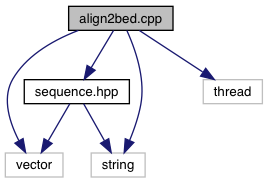
\includegraphics[width=273pt]{align2bed_8cpp__incl}
\end{center}
\end{figure}
\subsection*{Functions}
\begin{DoxyCompactItemize}
\item 
\mbox{\Hypertarget{align2bed_8cpp_ae66f6b31b5ad750f1fe042a706a4e3d4}\label{align2bed_8cpp_ae66f6b31b5ad750f1fe042a706a4e3d4}} 
int {\bfseries main} ()
\end{DoxyCompactItemize}


\subsection{Detailed Description}
Parsing D\+P\+GP. 

\begin{DoxyAuthor}{Author}
Anthony J. Greenberg
\end{DoxyAuthor}
Extracting S\+N\+Ps from the D\+P\+GP .seq files. The variant table will be in the {\itshape plink} B\+ED format. Each chromosome is processed by its own thread in parallel. 
\hypertarget{sequence_8cpp}{}\section{sequence.\+cpp File Reference}
\label{sequence_8cpp}\index{sequence.\+cpp@{sequence.\+cpp}}


Sequence and S\+NP file parsing and conversion.  


{\ttfamily \#include \char`\"{}sequence.\+hpp\char`\"{}}\newline
{\ttfamily \#include $<$vector$>$}\newline
{\ttfamily \#include $<$unordered\+\_\+map$>$}\newline
{\ttfamily \#include $<$string$>$}\newline
{\ttfamily \#include $<$iostream$>$}\newline
{\ttfamily \#include $<$fstream$>$}\newline
{\ttfamily \#include $<$limits$>$}\newline
{\ttfamily \#include $<$cmath$>$}\newline
Include dependency graph for sequence.\+cpp\+:\nopagebreak
\begin{figure}[H]
\begin{center}
\leavevmode
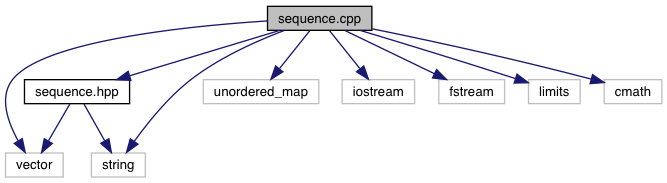
\includegraphics[width=350pt]{sequence_8cpp__incl}
\end{center}
\end{figure}


\subsection{Detailed Description}
Sequence and S\+NP file parsing and conversion. 

\begin{DoxyAuthor}{Author}
Anthony J. Greenberg 
\end{DoxyAuthor}
\begin{DoxyVersion}{Version}
0.\+9
\end{DoxyVersion}
Implementation of facilities that deal with common sequence and variant table file types. 
\hypertarget{sequence_8hpp}{}\section{sequence.\+hpp File Reference}
\label{sequence_8hpp}\index{sequence.\+hpp@{sequence.\+hpp}}


Sequence and S\+NP file parsing and conversion.  


{\ttfamily \#include $<$vector$>$}\newline
{\ttfamily \#include $<$string$>$}\newline
Include dependency graph for sequence.\+hpp\+:\nopagebreak
\begin{figure}[H]
\begin{center}
\leavevmode
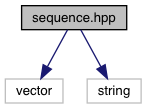
\includegraphics[width=182pt]{sequence_8hpp__incl}
\end{center}
\end{figure}
This graph shows which files directly or indirectly include this file\+:\nopagebreak
\begin{figure}[H]
\begin{center}
\leavevmode
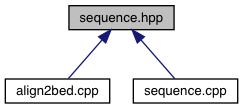
\includegraphics[width=254pt]{sequence_8hpp__dep__incl}
\end{center}
\end{figure}
\subsection*{Classes}
\begin{DoxyCompactItemize}
\item 
class \hyperlink{class_s_fparse}{S\+Fparse}
\begin{DoxyCompactList}\small\item\em Sequence file parsing class. \end{DoxyCompactList}\end{DoxyCompactItemize}


\subsection{Detailed Description}
Sequence and S\+NP file parsing and conversion. 

\begin{DoxyAuthor}{Author}
Anthony J. Greenberg 
\end{DoxyAuthor}
\begin{DoxyVersion}{Version}
0.\+9
\end{DoxyVersion}
Class definitions and interface documentation for facilities that deal with common sequence and variant table file types. 
%--- End generated contents ---

% Index
\backmatter
\newpage
\phantomsection
\clearemptydoublepage
\addcontentsline{toc}{chapter}{Index}
\printindex

\end{document}
